\documentclass[]{article}
\usepackage{graphicx}
\usepackage{subcaption}


%opening
\title{Multi-Phase Steel Micro-structure Segmentation using UNet: Generalization and Magnification Independence Analysis}
\author{[Early Draft]}

\begin{document}

\maketitle

\begin{abstract}
	
The micro-structures of advanced high-strength steel, including constituents such as Martensite, Ferrite, and Bainite, provide crucial insights into the steel's physical properties, but while their manual examination is laborious and prone to subjective bias the other alternatives are cost-prohibitive. Our proposed methodology involves the use of a UNet model to perform image segmentation of steel microstructures, automating the traditionally manual analysis process. This model requires a minimal amount of annotated micrographic images for training, yet it demonstrates excellent performance in segmenting steel microstructures. Importantly, our approach tries to maintain its accuracy across different magnifications and various types of steel, highlighting its versatility and generalizability. This paper contributes to the advancement of industrial processes by offering a scalable, efficient, and objective solution for the characterization of microstructures, significantly improving the metallographic segmentation process in the steel industry.

\end{abstract}

\section{Introduction}

The advent of Artificial Intelligence (AI) has brought about transformative changes across various sectors, including manufacturing processes \cite{russel2010}. AI systems, by encapsulating significant knowledge into models, have become an indispensable component of the Industry 4.0 revolution \cite{lasi2014industry}. In this scenario, the segmentation of metallographic images is pivotal for understanding material characteristics and refining manufacturing procedures, thereby enhancing product quality assessment and fostering the creation of new products \cite{gonzalez2008digital, cv_algandapp}.

Among the various applications in industrial manufacturing, our focus is on the segmentation of metallographic images. Image segmentation, a fundamental problem in computer vision, involves dividing an image into distinct regions based on specific criteria \cite{HARALICK1985100}. This problem has been extensively studied and finds applications in numerous domains, including medical image analysis \cite{Litjens_2017, shen2017}, autonomous driving \cite{chen2017deeplab}, and robotics \cite{garciagarcia2017review}.

Transformation-induced-plasticity (TRIP) effect, is a material phenomenon that occurs in multi-phase microstructures of steel plates. The TRIP effect involves the transformation of retained austenite to martensite during plastic deformation, leading to a significant increase in the work-hardening rate \cite{tripSteels}. This transformation strengthens the neck region, delaying further deformation and enhancing the strength-ductility balance \cite{ALLAIN2004158}. Harnessing the TRIP effect in advanced high-strength steels (AHSS) has emerged as a significant strategy for the steel and automotive industries to maintain high strength and safety properties, while also addressing critical environmental concerns such as fuel consumption and air pollution \cite{BOUAZIZ2011141}. So it becomes essential to find the proper structures of the parts that underwent TRIP effect to access the quality of the produced AHSS. One of the ways to finding the structures in the steel to use obtain images using a Scanning Electron Microscope (SEM) and then generate corresponding labels using methods like Electron Backscatter Diffraction (EBSD). Despite its effectiveness, relying solely on EBSD for routine quality assessment presents several challenges. First, EBSD is not only time-consuming and labor-intensive, but it is also cost-prohibitive for large-scale or frequent analysis. Moreover, while EBSD provides detailed crystallographic information, its resolution is often lower compared to SEM, thus limiting its utility for fine-detail microstructural analysis. Given these challenges, there is a compelling need for alternative, more efficient methods for microstructure characterization. This is where AI-driven image segmentation, specifically using the UNet model, can offer significant advantages. UNet has been widely successful in various domains for its ability to yield precise segmentation, even with fewer training images. Its architecture is particularly suited for biomedical image segmentation, and we extend its application for the segmentation of SEM images of steel microstructures.

However, the segmentation of microscopic steel images is a challenging task due to the intricate nature of steel microstructures and the similarity in appearance among different components when observed under varying magnifications. Unlike general image segmentation problems where objects have distinct boundaries, the components in steel microstructures often exhibit subtle differences and complex structures that require careful analysis for accurate segmentation \cite{NIPS2012_imagenet}. Steel microstructures contain critical information about the mechanical properties and quality of the material, making it essential to accurately separate and identify the different components. This level of detail and precision is particularly crucial in applications such as additive manufacturing, quantitative analysis, and quality control.

Despite the significance of steel image segmentation, there is a scarcity of research specifically addressing this challenge. The existing literature in the field of metallographic segmentation predominantly focuses on limited datasets, where the models are trained and tested on the same set of data, limiting their generalizability. Moreover, previous methods often fail to capture the fine-detailed microstructures, impeding their practical utility in real-world applications \cite{LeCun2015, GoodBengCour16}.

In this study, we propose a scalable metallographic segmentation solution that leverages deep learning techniques and incorporates different augmentation strategies to overcome the limitations of traditional methods. By training on a known set of inputs and testing on diverse magnified images and steel types, our approach aims to provide accurate and detailed segmentation results, advancing the field of steel image analysis and supporting industrial applications in a more robust and comprehensive manner. Our proposed approach has several advantages. First, it substantially reduces the time and cost associated with microstructure characterization, as compared to EBSD. Second, it allows for high-resolution, detailed segmentation of microstructures, given the superior resolution of SEM images. Lastly, it enables large-scale, routine analysis of steel microstructures, thus facilitating regular quality assessment and control in industrial applications. EBSD still remains necessary for generating ground truth labels for SEM images and for occasional validation of segmentation results.

The subsequent sections of this paper elaborate on our proposed methodology and present experimental results demonstrating its effectiveness in automating microstructure characterization. Section 2 reviews related works in the domain. Section 3 discusses the characteristics and challenges of microstructure segmentation, as well as the UNet architecture and dataset. Section 4 presents the methodology, including model architecture, augmentations, and training process. Section 5 focuses on experimentation, covering evaluation metrics, experimental setup, and results on both training and inference images. Section 6 provides a detailed discussion and analysis of the experimental results, addressing challenges, limitations, and factors influencing performance variations. Finally, section 7 concludes by summarizing the key findings, emphasizing the importance of accurate microstructure segmentation, and suggesting future research directions.

\section{Related Works}

The application of deep learning techniques, particularly convolutional neural networks (CNNs), has shown promising results in various image segmentation tasks. The UNet architecture, a type of CNN, has been widely used for medical image segmentation due to its ability to capture both local and global context by using a symmetric encoder-decoder structure \cite{cao2021swinunet}.

In the realm of microstructure segmentation, previous studies have explored various methodologies to achieve accurate classification and segmentation results. Velichko et al. proposed a method based on data mining techniques, specifically extracting morphological features and utilizing a feature classification step using Support Vector Machines (SVMs). This approach was applied to cast iron and demonstrated the potential of machine learning in microstructural analysis \cite{sym13071176}. However, this method, while effective for simpler microstructures, may not be as efficient for complex steel microstructures due to the intricate nature and the subtle differences among different components.

Similarly, Pauly et al. adopted a similar approach on a contrasted and etched dataset of steel acquired through SEM and LOM imaging \cite{LAI2009665}. However, the results yielded a relatively low accuracy of 48.89\% in microstructural classification due to the complex nature of substructures and the lack of discriminative features. This highlights the need for a more robust and efficient method for microstructure segmentation.

Durmaz et al. proposed a multidisciplinary deep learning approach that equally considers specimen preparation and imaging \cite{Durmaz2021}. They trained distinct UNet architectures with 30-50 micrographs of different imaging modalities and electron backscatter diffraction-informed annotations. The study focused on the challenging task of lath-bainite segmentation in complex-phase steel, achieving accuracies of 90\% that rival expert segmentations. While this approach has shown promising results, it requires a large number of annotated images for training, which may not always be feasible in practical scenarios.

In contrast to these previous works, our proposed method aims to provide a scalable solution that requires only a small number of annotated images for training. We leverage different augmentation strategies to increase the diversity of our training data, thereby enhancing the robustness and generalizability of our model. Furthermore, our approach is designed to handle different magnified images and steel types, making it more versatile and applicable to a wider range of scenarios.

In summary, while previous studies have made significant contributions to the field of microstructure segmentation, our work aims to address the limitations of these methods by proposing a scalable, efficient, and versatile solution for steel microstructure segmentation.

\section{Background}
This section provides an overview of the key aspects of the semantic segmentation problem in the context of microstructures. It also discusses the dataset utilized in this study and highlights the associated challenges.
\subsection{Characteristics and Challenges of Microstructure Segmentation}
Segmenting microstructures in metallographic images presents a highly challenging task due to the distinctive visual characteristics inherent in these images.

Microstructure segmentation in microscopic steel images is complex due to several factors. Firstly, these images contain high-resolution details that necessitate precise detection and segmentation of fine-grained structures. Furthermore, the inherent variability in textures and shapes within these images adds to the challenge of accurately distinguishing and segmenting different regions. Additionally, imbalanced class distributions, where some components are more prevalent than others, introduce difficulties in achieving accurate segmentation results across all classes. Moreover, the absence of landmark information in these images limits the availability of unique characteristics that could aid in capturing the distinct features of microstructures \cite{LUENGO2022232}.

Due to the heterogenous material properties in these metallographic images, accurately delineating and classifying different regions becomes difficult. Heterogenous properties also heighten the variations in scale and magnification, leading to changes in the appearance and size of the microstructures.

While manual annotation of metallographic images is a labor-intensive and time-consuming, producing EBSD images is cost-prohibitive and not suitable for more frequent analysis. As a result, there is a scarcity of large, labeled datasets specifically tailored for microstructure segmentation \cite{Roberts2019}. This limitation hinders the application of supervised learning methods, which typically require ample training data to achieve optimal performance.

\subsection{Why UNet: An Ideal Choice for Microstructure Segmentation}

The choice of an appropriate model is crucial for achieving accurate results in steel image segmentation. Given the challenges specific to steel microstructure segmentation, we selected the UNet architecture \cite{ronneberger2015unet} for its suitability.

UNet, a convolutional neural network (CNN) architecture, has demonstrated exceptional performance in segmentation tasks, particularly in capturing fine details and handling varying scales of structures. It was originally designed for biomedical image segmentation, where the availability of annotated training data is often limited, and the need for detailed segmentation is high. These characteristics make UNet an ideal choice for the segmentation of steel microstructures.The UNet architecture is characterized by its U-shaped design, which consists of a contracting path to capture context and a symmetric expanding path that allows precise localization. This design enables the model to preserve fine-grained details while capturing global context, making it suitable for steel microstructure segmentation. Another key feature of UNet is the incorporation of skip connections, which allow the fusion of features from multiple scales. This enhances the model's ability to capture intricate details and accurately segment complex structures, a crucial requirement in steel microstructure segmentation.
Furthermore, UNet is designed to work with very few training images and yields more precise segmentations. This is particularly beneficial in our case, where the availability of pixel-wise labels generated through EBSD is limited.

\subsection{Dataset}

The dataset leveraged in our study consists of six E-type steel images captured through a Scanning Electron Microscope (SEM). Due to the minuscule size of the phases in this type of steel, using optical microscopy (OM) for image capture is ineffective. Thus, SEM provides the necessary resolution and detail for effective analysis.

Corresponding to each SEM image, we generated ground truth labels using Electron Backscatter Diffraction (EBSD), providing precise information about the distinct components and phases present within the steel microstructures. In total, the dataset contains images belonging to three different classes, each corresponding to a different phase of the steel microstructure. The labeling colors for each class are as follows:
\begin{itemize}
	\item Orange: Ferrite
	\item Purple: Bainite
	\item Yellow: Martensite
\end{itemize}

The steel used in this study is termed 590DP, which signifies a dual-phase steel with a tensile strength of 590MPa. This kind of steel, also known as gigasteel when the tensile strength reaches 1GPa, is classified as ultra-high-strength steel and is commonly used in automotive applications due to its exceptional strength and formability.

Labeling of the SEM images was accomplished using a superpixel labeling method. Superpixel segmentation groups pixels into larger, coherent superpixels based on similarity in color, texture, and other factors, thus providing a more efficient and accurate labeling process for our dataset. This approach, coupled with the precision of SEM imaging and the detailed phase information from EBSD, ensures the creation of a robust and comprehensive dataset for training and testing our UNet segmentation model.

\begin{figure}[ht]
	\centering
	\begin{subfigure}[b]{0.45\textwidth}
		\centering
		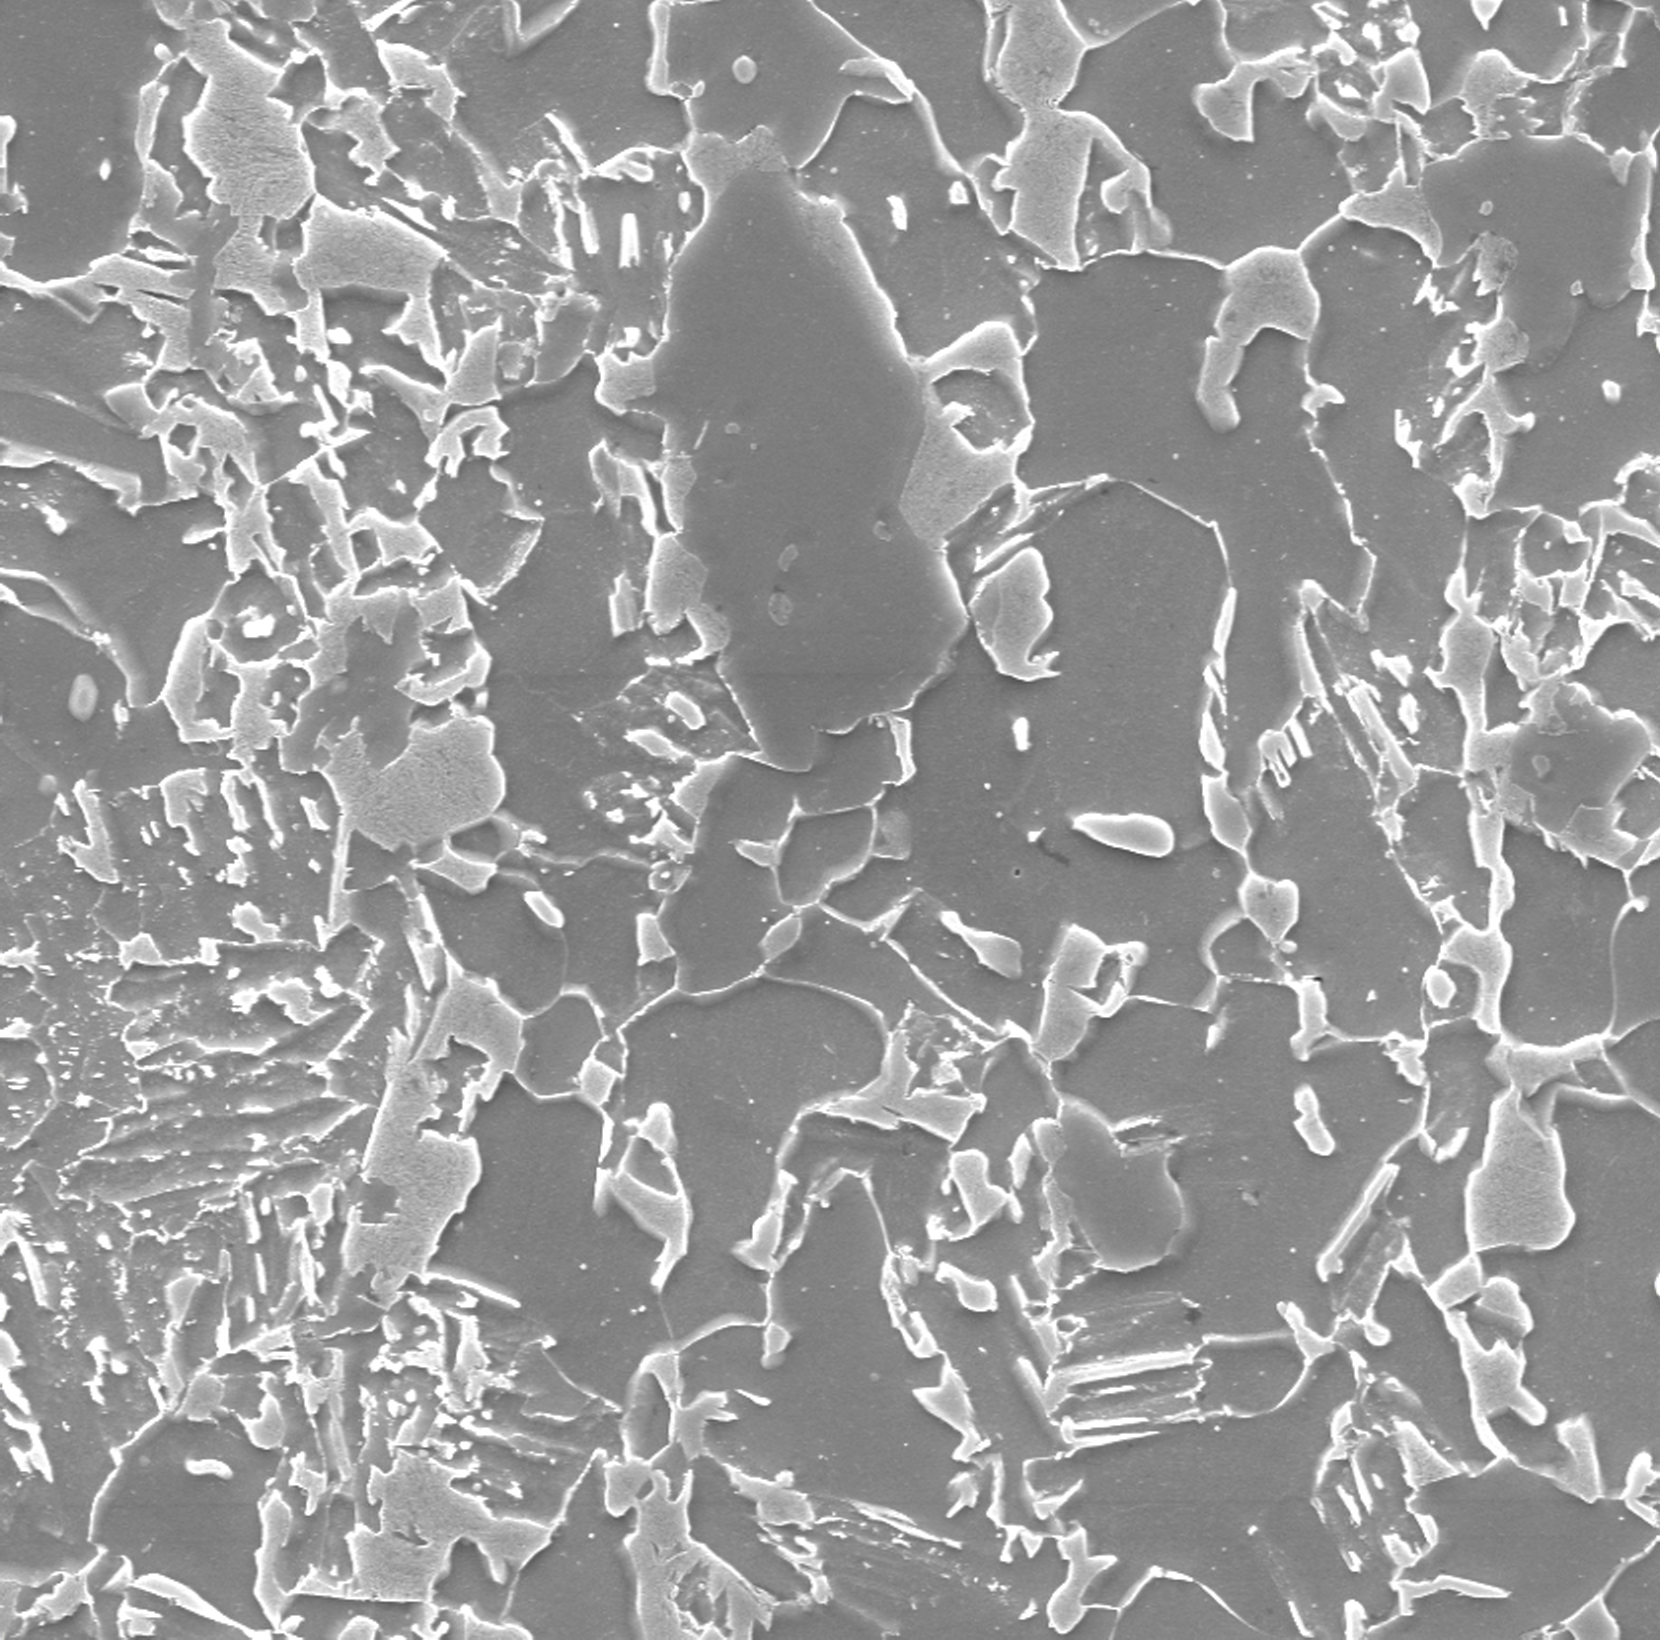
\includegraphics[width=\textwidth]{images/1.png}
		\caption{SEM image}
		\label{fig:image1}
	\end{subfigure}
	\hfill
	\begin{subfigure}[b]{0.45\textwidth}
		\centering
		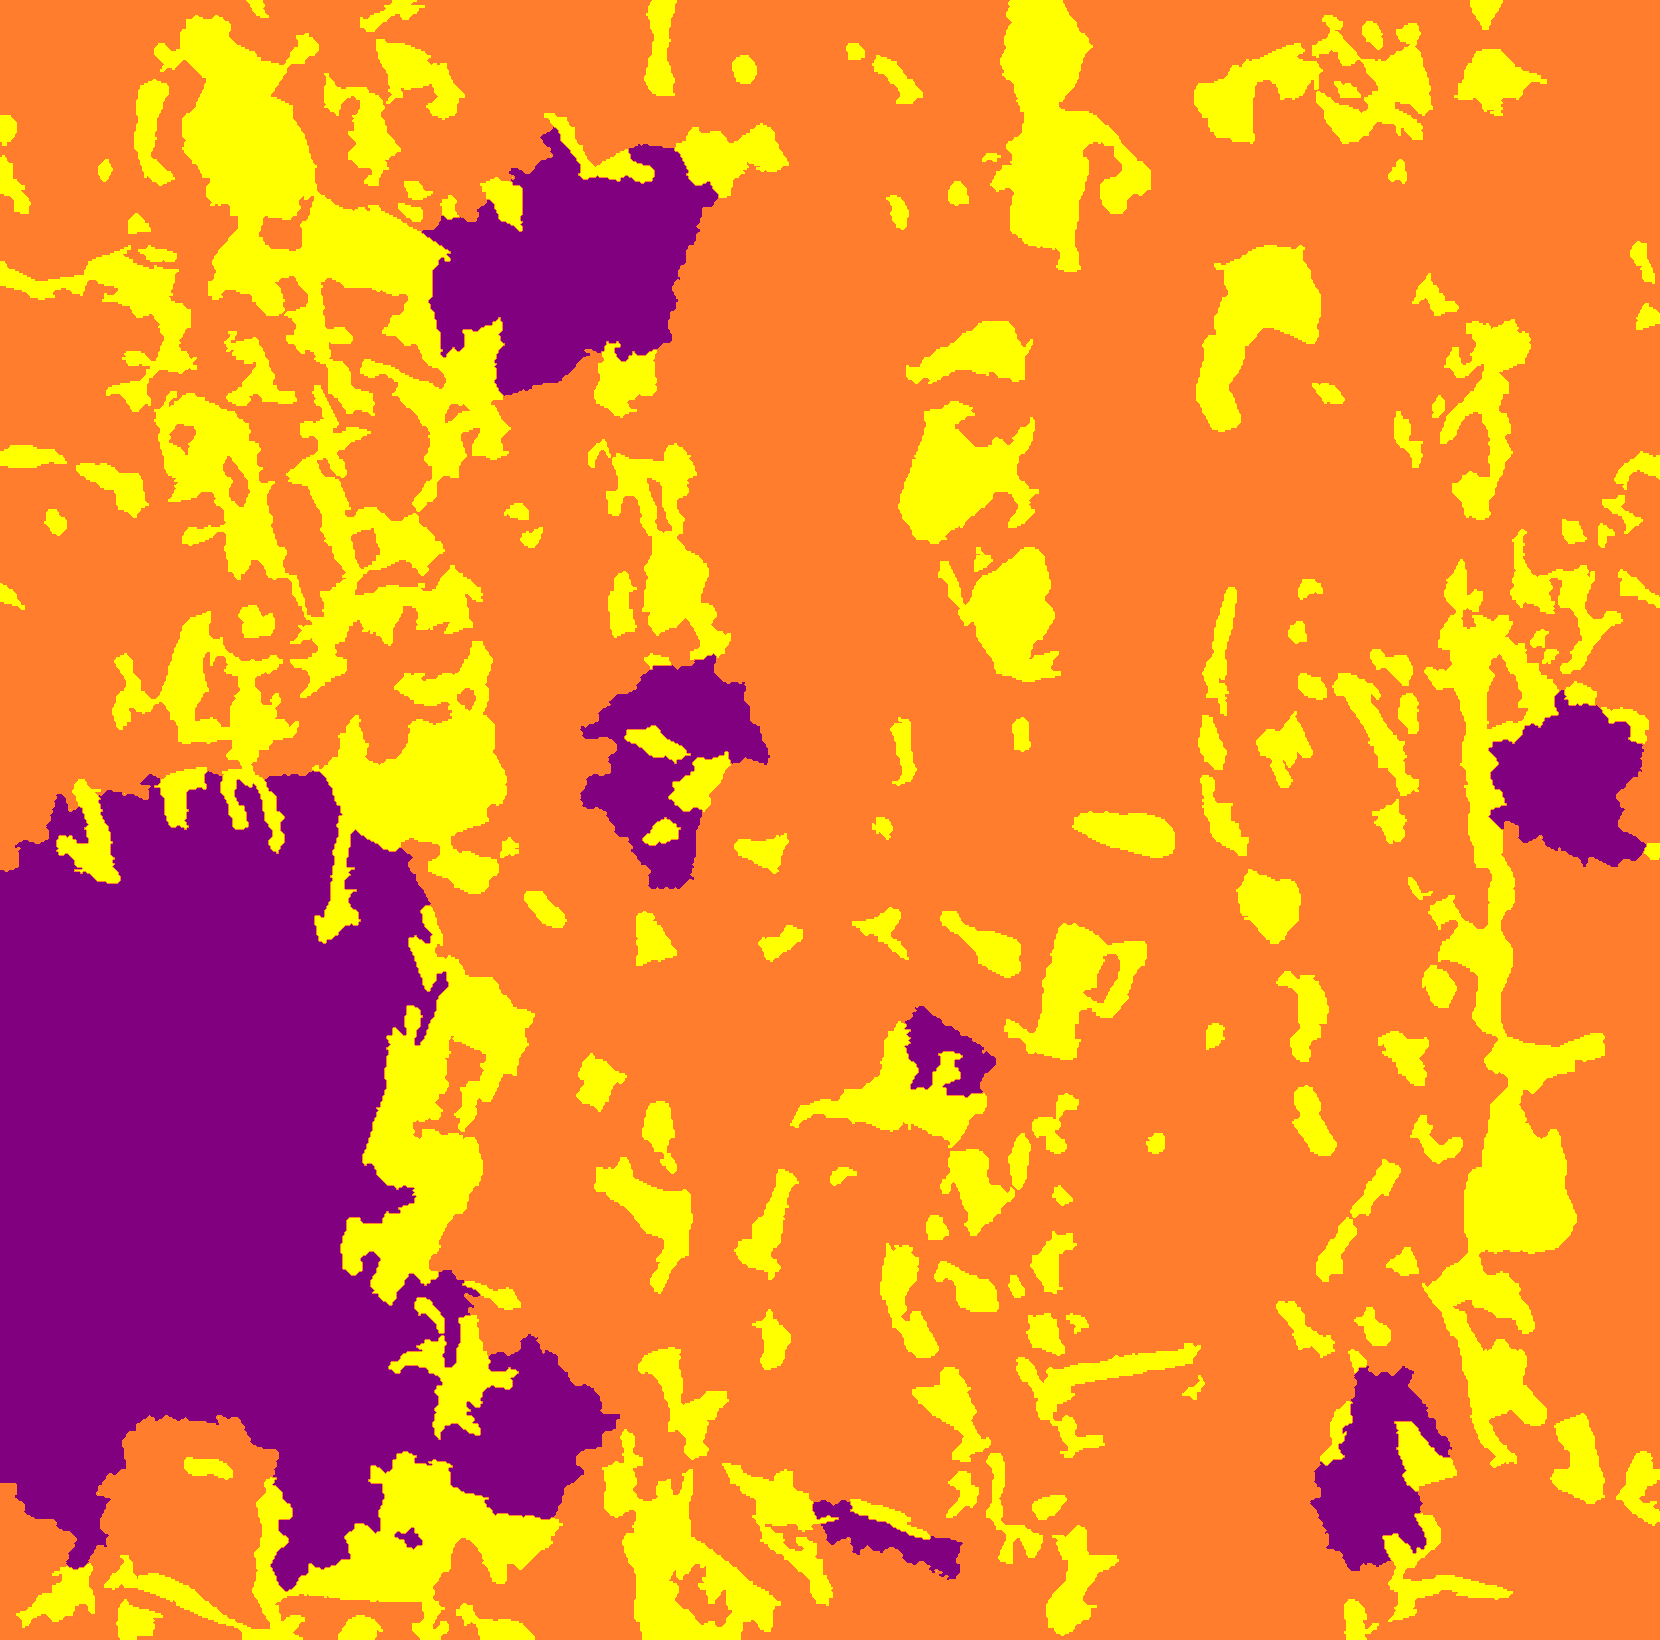
\includegraphics[width=\textwidth]{images/1_label.png}
		\caption{EBSD and Superpixel labeling }
		\label{fig:image2}
	\end{subfigure}
	\caption{x2700 magnified E-type steel image and its corresponding label}
	\label{fig:combined}
\end{figure}


In the training phase of our study, we utilized five out of the six E-type steel images to augment and train the UNet model. The remaining image served as an initial testing ground to validate the model's learning.

To evaluate the model's performance and its ability to generalize, we extended our testing to include steel images magnified at higher magnifications of 3000x and 5000x. The ability to accurately segment images at these higher magnifications is crucial, as it enables the detailed analysis of complex microstructures that are typically observed at these scales.

Furthermore, to test the model's versatility and its effectiveness across various steel types, our testing dataset was expanded to include images of A-type, H2-type, and D3-type steels. These additional steel types have unique microstructural characteristics that pose different challenges to image segmentation. By testing the model across these diverse types of steel, we aim to validate its robustness and its potential for broad applicability in industrial settings.

\begin{figure}[ht]
	\centering
	\begin{subfigure}[b]{0.2\textwidth}
		\centering
		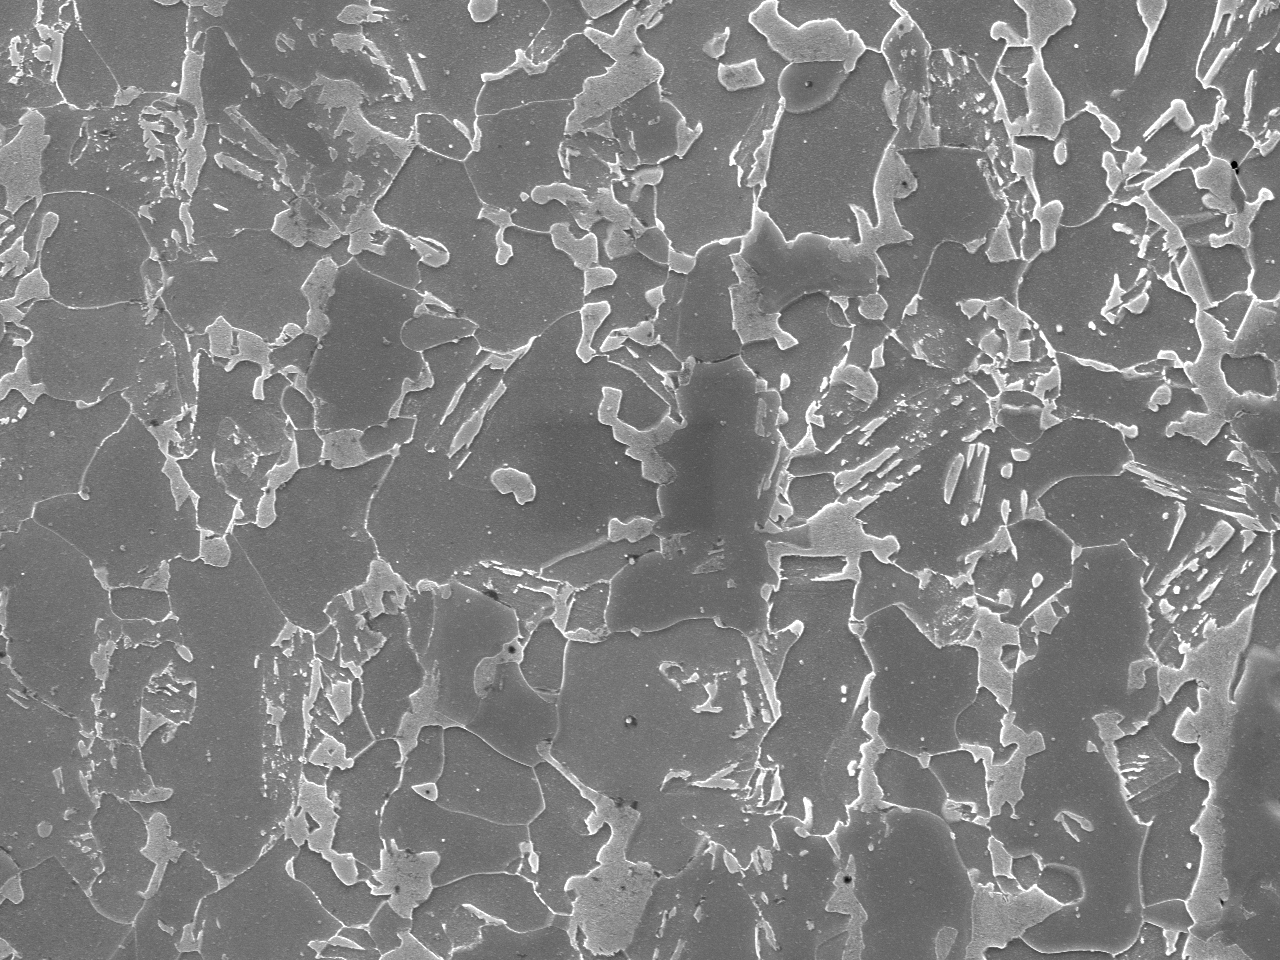
\includegraphics[width=\textwidth]{images/x3000/1.png}
		\caption{x3000 SEM}
		\label{fig:image2.1.1}
	\end{subfigure}
	\begin{subfigure}[b]{0.2\textwidth}
		\centering
		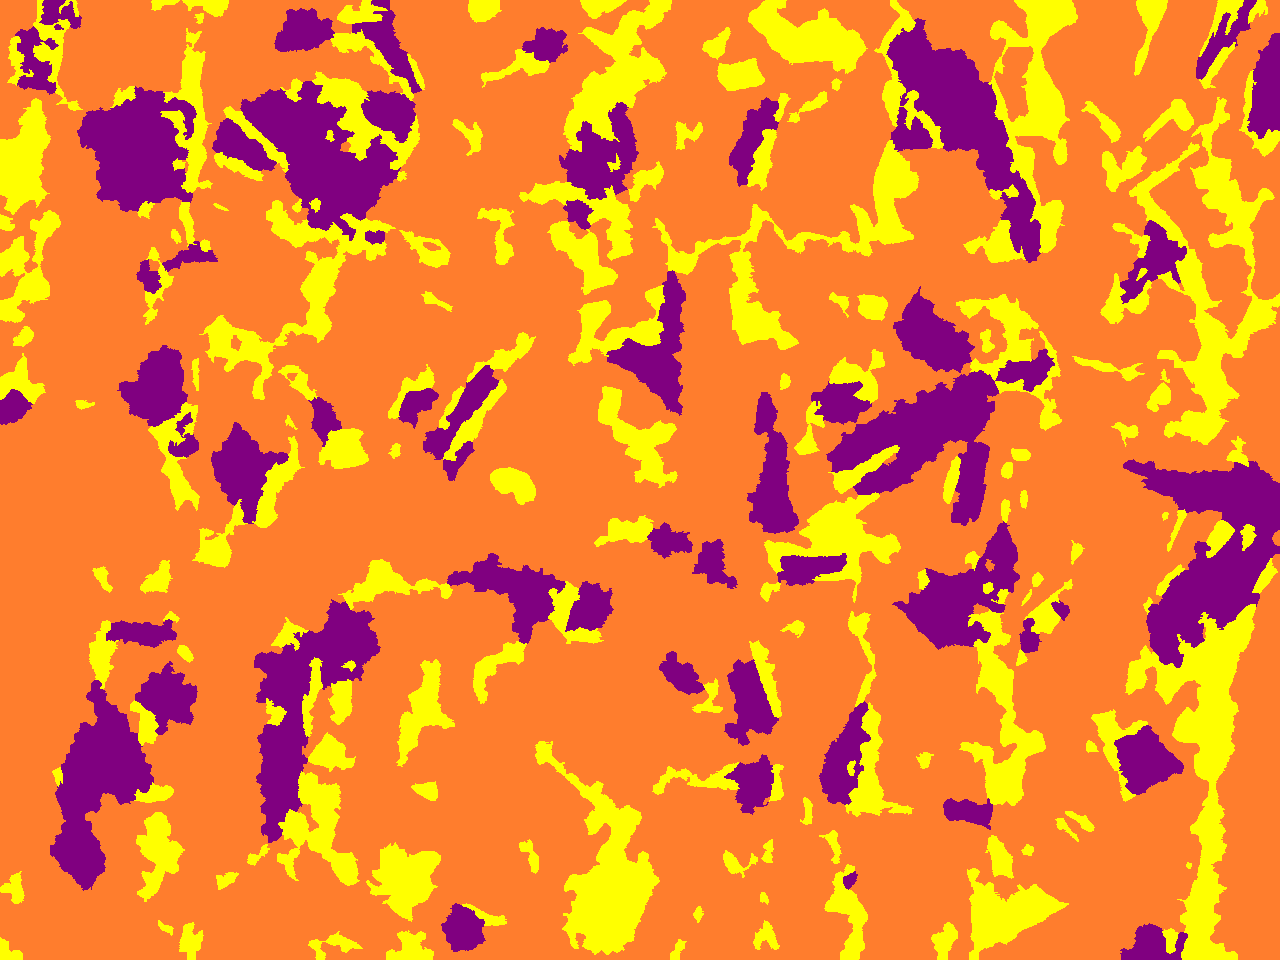
\includegraphics[width=\textwidth]{images/x3000/1_label.png}
		\caption{x3000 label}
		\label{fig:image2.1.2}
	\end{subfigure}
	\hfill
	\begin{subfigure}[b]{0.2\textwidth}
		\centering
		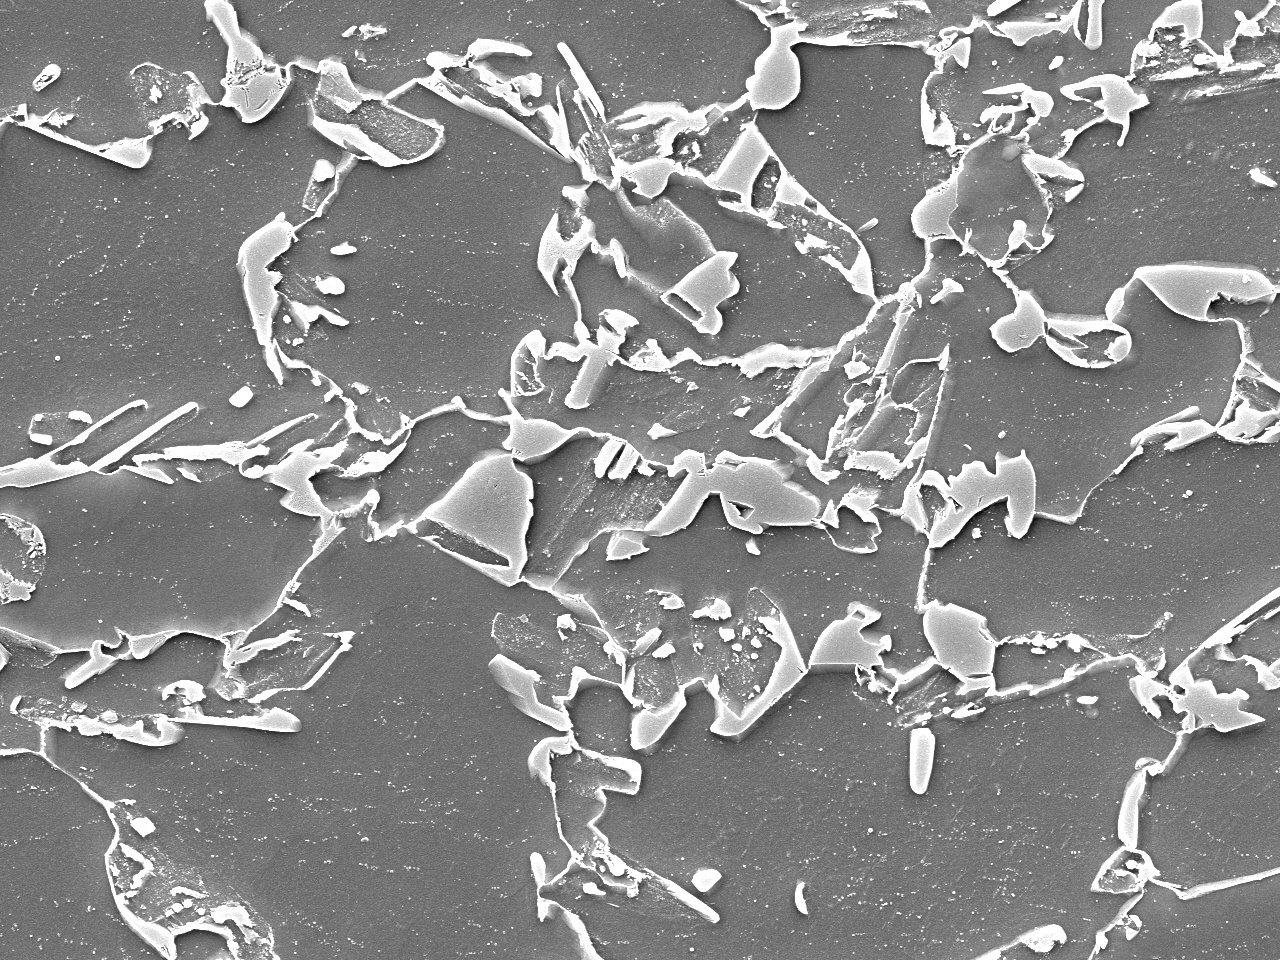
\includegraphics[width=\textwidth]{images/x5000/1.png}
		\caption{x5000 SEM}
		\label{fig:image2.2.1}
	\end{subfigure}
	\begin{subfigure}[b]{0.2\textwidth}
		\centering
		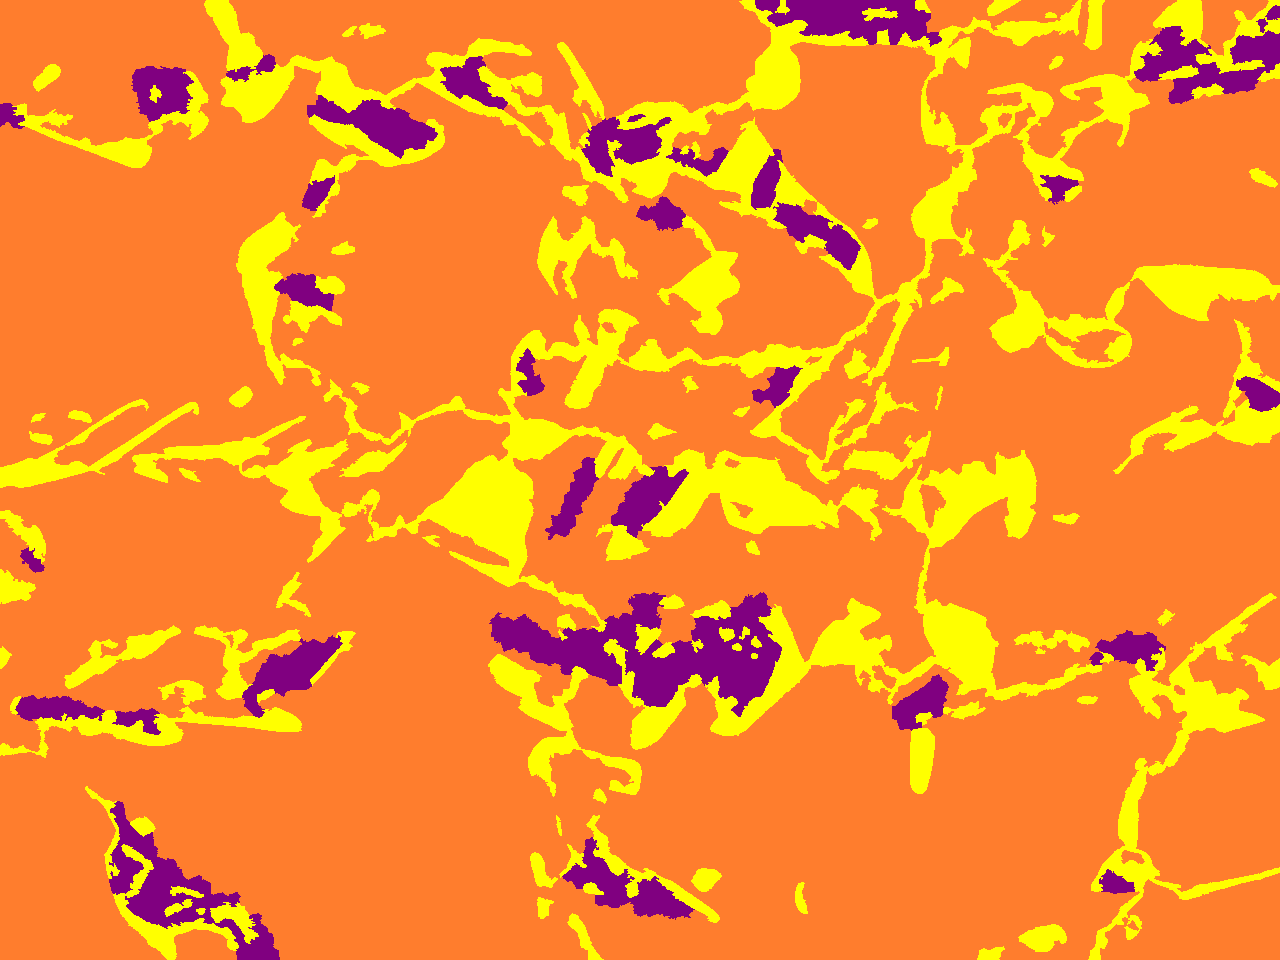
\includegraphics[width=\textwidth]{images/x5000/1_label.png}
		\caption{x5000 label}
		\label{fig:image2.2.2}
	\end{subfigure}
	
	\begin{subfigure}[b]{0.2\textwidth}
		\centering
		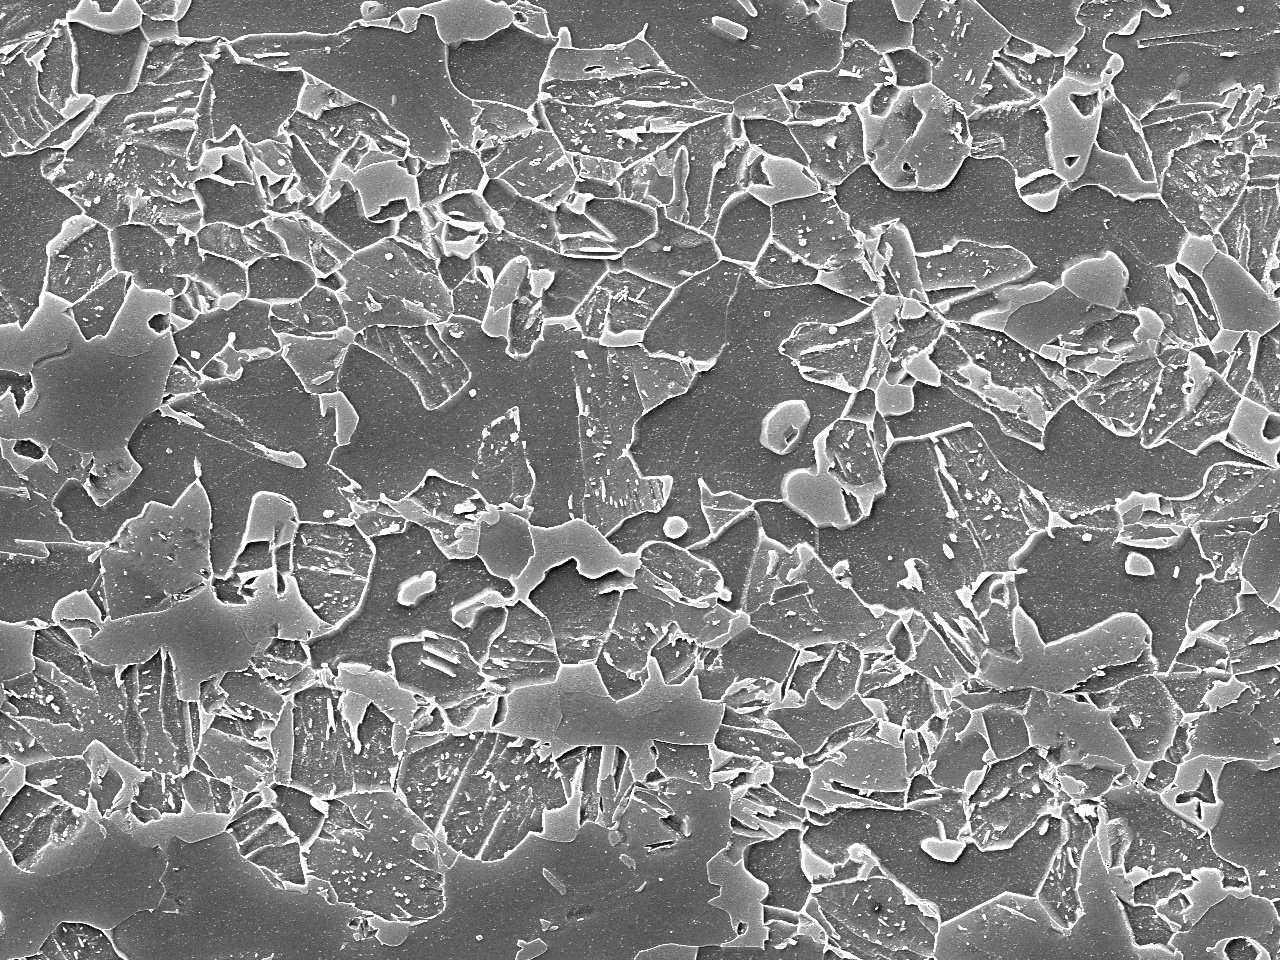
\includegraphics[width=\textwidth]{images/A-type/1.png}
		\caption{A-type SEM}
		\label{fig:image2.3.1}
	\end{subfigure}
	\begin{subfigure}[b]{0.2\textwidth}
		\centering
		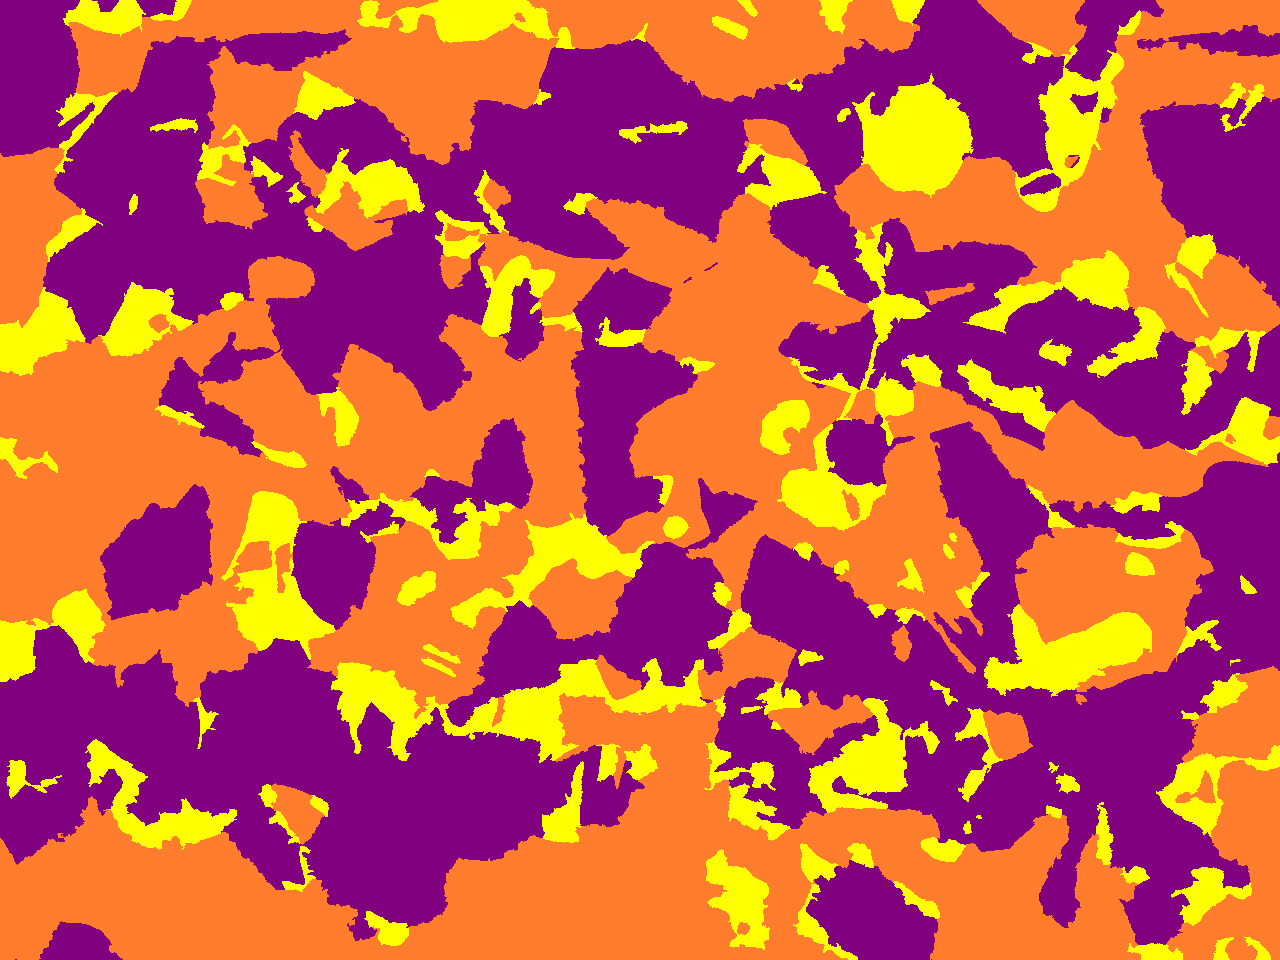
\includegraphics[width=\textwidth]{images/A-type/1_label.png}
		\caption{A-type label}
		\label{fig:image2.3.2}
	\end{subfigure}
	\hfill
	\begin{subfigure}[b]{0.2\textwidth}
		\centering
		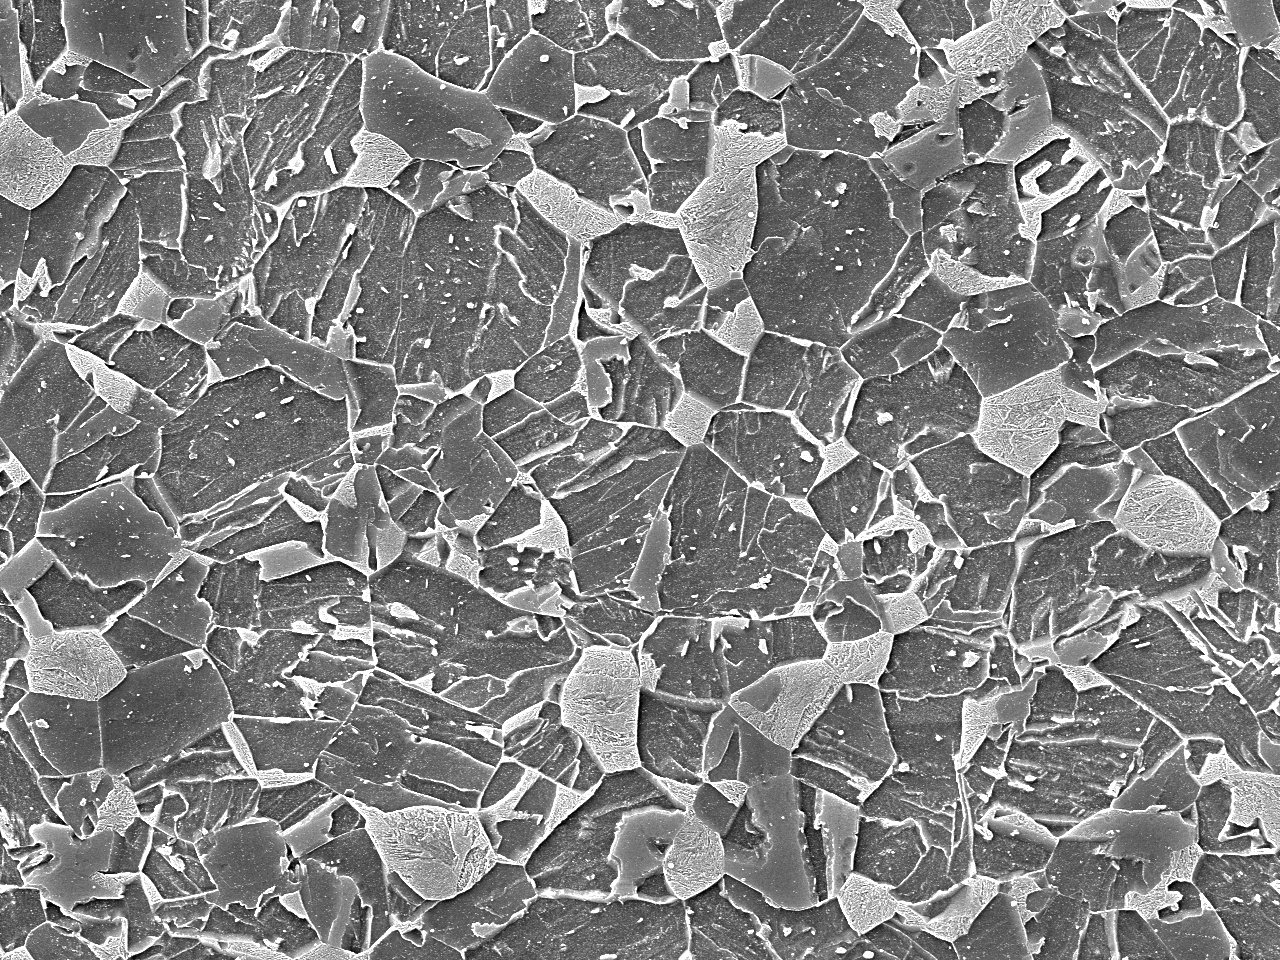
\includegraphics[width=\textwidth]{images/D3-type/1.png}
		\caption{D3-type SEM}
		\label{fig:image2.4.1}
	\end{subfigure}
	\begin{subfigure}[b]{0.2\textwidth}
		\centering
		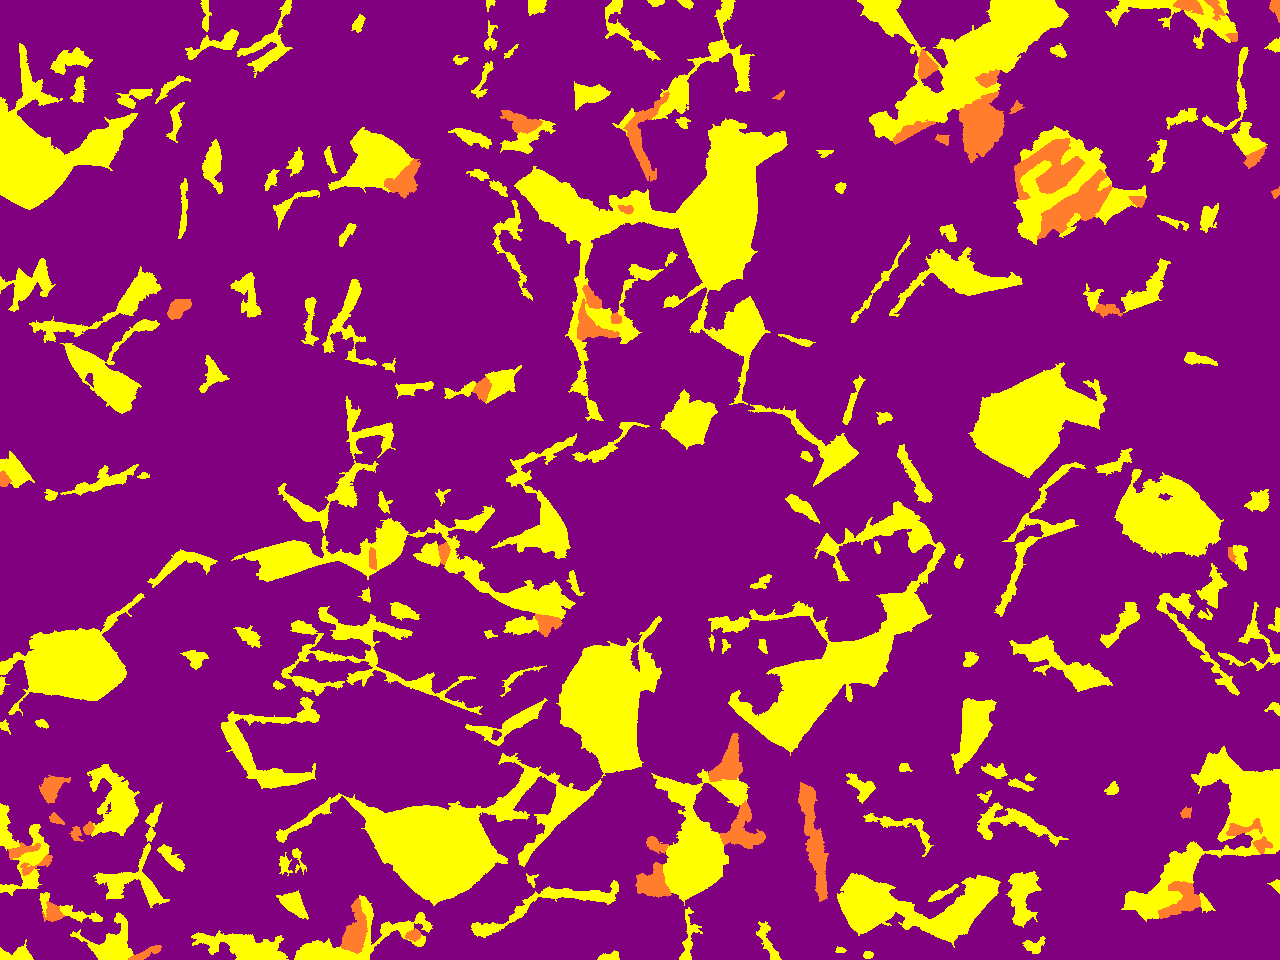
\includegraphics[width=\textwidth]{images/D3-type/1_label.png}
		\caption{D3-type label}
		\label{fig:image2.4.2}
	\end{subfigure}
	
	\begin{subfigure}[b]{0.2\textwidth}
		\centering
		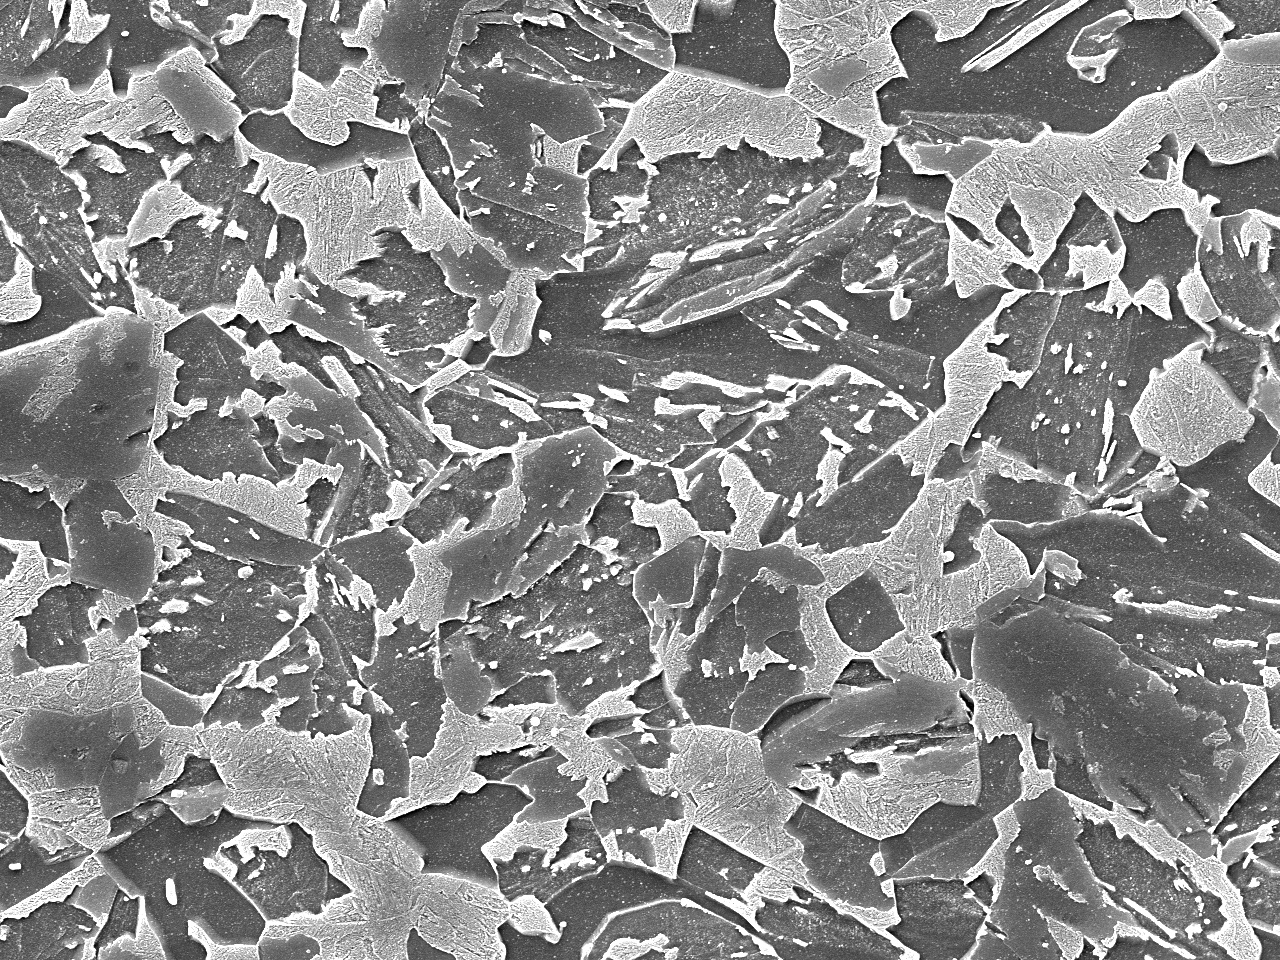
\includegraphics[width=\textwidth]{images/H2-type/1.png}
		\caption{H2-type SEM}
		\label{fig:image2.5.1}
	\end{subfigure}
	\begin{subfigure}[b]{0.2\textwidth}
		\centering
		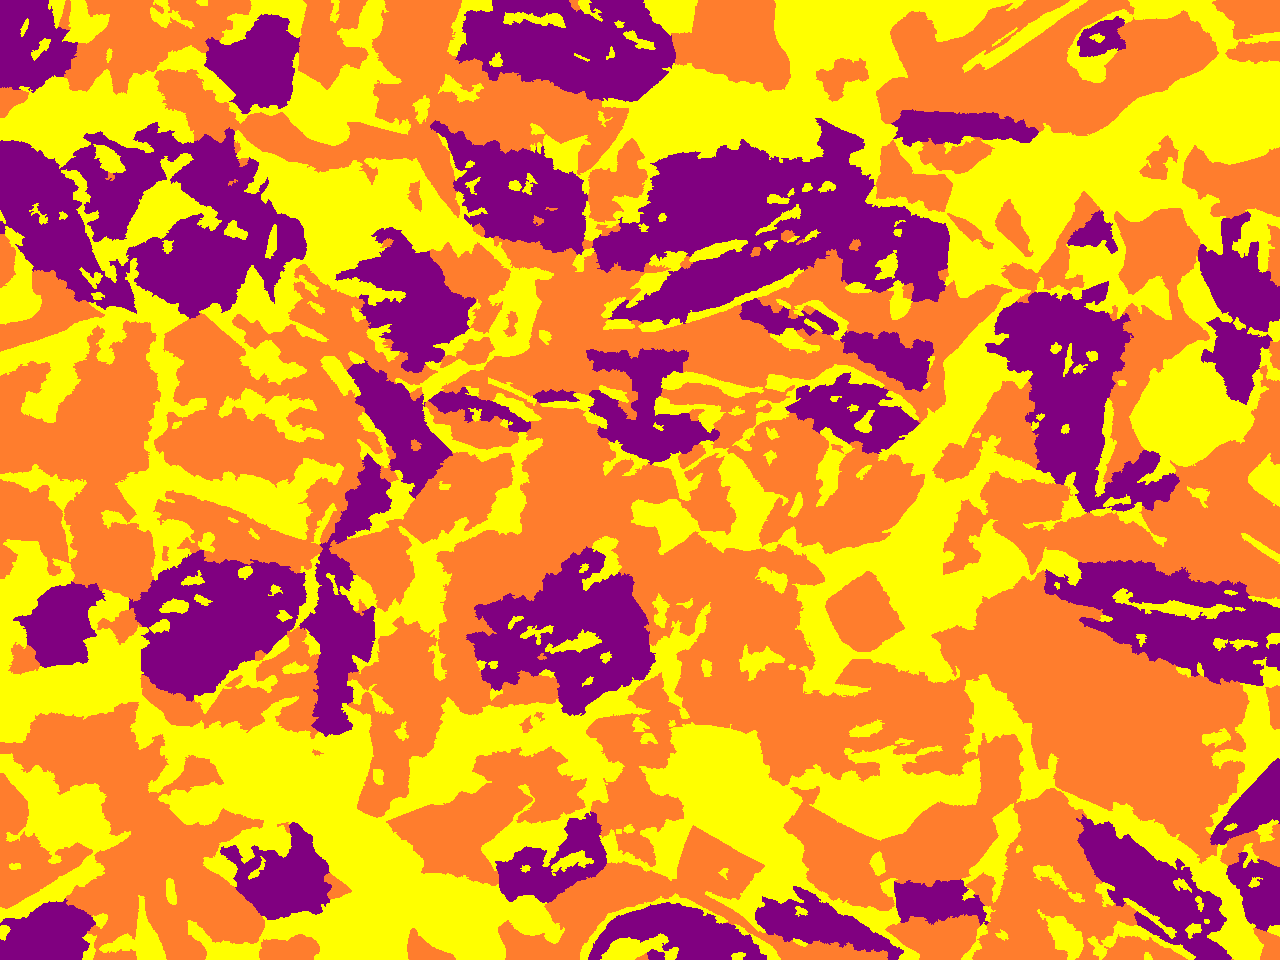
\includegraphics[width=\textwidth]{images/H2-type/1_label.png}
		\caption{H2-type label}
		\label{fig:image2.5.2}
	\end{subfigure}
	\caption{Sample images of various steel and magnification types used during inference.}
	\label{fig:combined}
\end{figure}

It's worth emphasizing that the images magnified at 3000x and 5000x originate from the same E-type steel that was used to train our model. This inclusion demonstrates the model's capacity to effectively scale across varied magnification levels, maintaining its segmentation accuracy even at high magnifications that reveal more intricate microstructures.

Furthermore, the incorporation of A-type, D3-type, and H2-type steel images, all magnified at 5000x, underscores the model's capability to generalize across different steel types. Despite these steel types featuring distinct microstructural characteristics compared to the E-type steel used in training, the model is able to accurately identify and segment their microstructures. This ability to generalize over various steel types suggests the model's potential for broad applicability in real-world industrial contexts, well beyond its initial training data.

\section{Methodology}
In the following section, we detail the methodology used in our study, which is designed to address the challenges associated with the segmentation of steel microstructures. The core of our approach involves three key components: the model architecture, the augmentation strategies, and the training process.

\subsection{Model Architecture}


\bibliography{reference}
\bibliographystyle{plain}
\end{document}
